\documentclass{beamer}
%\documentclass{beamer}

%------------
%  Themes
%------------
%\usepackage{beamerthemeshadow}
%\usepackage{beamerthemebars}
%\usepackage{beamerthemeclassic}
%\usepackage{beamerthemelined}
%\usepackage{beamerthemesidebar}
%\usepackage{beamerthemesplit}
%\usepackage{beamerthemetree}
%-----------------------------
%\usepackage{beamerthemeAnnArbor}
%\usepackage{beamerthemePaloAlto}
\usepackage{beamerthemeCambridgeUS}
%\usepackage{beamerthemeAntibes}
%\usepackage{beamerthemeBergen}
%\usepackage{beamerthemeBerkeley}
%\usepackage{beamerthemeBerlin}
%\usepackage{beamerthemeGoettingen}
%\usepackage{beamerthemeHannover}
%\usepackage{beamerthemeMarburg}
%\usepackage{beamerthemeMontpellier}
%\usepackage{beamerthemeSingapore}
%\usepackage{beamerthemeSzeged}
%\usepackage{beamerthemeWarsaw}

%------------
%  Colors
%------------
%\usepackage{beamercolorthemecrane}
%\usepackage{beamercolorthemedolphin}
%\usepackage{beamercolorthemeseahorse}
%\usepackage{beamercolorthemewolverine}

%------------
%  Outer Themes
%------------
%\usepackage{beamerouterthemeinfolines}
%\usepackage{beamerouterthememiniframes}
%\usepackage{beamerouterthemeshadow}
%\usepackage{beamerouterthemesidebar}
%\usepackage{beamerouterthemesmoothbars}
%\usepackage{beamerouterthemesmoothtree}
%\usepackage{beamerouterthemesplit}
%\usepackage{beamerouterthemetree}

%------------
%  Inner Themes
%------------
%\usepackage{beamerinnerthemecircles}
%\usepackage{beamerinnerthemedefault}
%\usepackage{beamerinnerthemeinmargin}
%\usepackage{beamerinnerthemerectangles}
%\usepackage{beamerinnerthemerounded}

%------------
%  Fonts
%------------
%\usepackage{beamerfontthemedefault}
%\usepackage{beamerfontthemeserif}
%\usepackage{beamerfontthemestructureitalicserif}
%\usepackage{beamerfontthemestructurebold}
%\usepackage{beamerfontthemestructuresmallcapsserif}

%commented this next command out to get it all to work.
%\beamertemplateshadingbackground{red!10}{yellow!10}

%\beamertemplatetransparentcovereddynamic
%\beamertemplatetransparentcovered

\usenavigationsymbolstemplate

\usepackage{pgf,pgfarrows,pgfnodes,pgfautomata,pgfheaps,pgfshade}
\usepackage{epic}
\usepackage{graphicx}
\usepackage{geometry}
\usepackage{amsmath,amssymb,bm}
\usepackage[latin1]{inputenc}
\usepackage{colortbl}
\usepackage[english]{babel}
\usepackage{soul}
\usepackage{curves}
\usepackage{multirow}
\usepackage{pgf}
\usepackage{xspace}
\usepackage[absolute,overlay]{textpos}
\usepackage{multimedia}
\usepackage{array}
%\usepackage{cite}
\usepackage{verbatim}
\usepackage[style=ieee]{biblatex}
\usepackage{caption}

\graphicspath{{fig/}{./}}

%\definecolor{NavyBlue}{rgb}{0,0,0.9019}
\definecolor{Red}{rgb}{.9,0.2,0.2}
\definecolor{Maroon}{rgb}{0.6,0.05,0.03}
\definecolor{Verde}{rgb}{0,0.7019,0.3519}
%\definecolor{Marron}{rgb}{0.5019,0.5019,0}
%\definecolor{Bege}{rgb}{0.8837,0.8274,0.3921}
%\definecolor{Blue}{rgb}{0,0,1}
%\definecolor{Green}{rgb}{0,0.6019,0.4019}
\definecolor{Gray}{rgb}{0.3,0.3,0.3}

\definecolor{NavyBlue}{rgb}{0,0,0.9019}
%\definecolor{Red}{rgb}{.9,0.2,0.2}
%\definecolor{Maroon}{rgb}{0.6,0.05,0.03}
%\definecolor{Verde}{rgb}{0,0.6019,0.4019}
%\definecolor{Marron}{rgb}{0.5019,0.5019,0}
%\definecolor{Bege}{rgb}{0.8837,0.8274,0.3921}
%\definecolor{Blue}{rgb}{0,0,1}
%\definecolor{Green}{rgb}{0,0.7019,0.3019}
%\definecolor{Gray}{rgb}{0.3,0.3,0.3}

\setbeamertemplate{headline}{}
\setbeamertemplate{itemize items}[default]
\setbeamertemplate{enumerate items}[default]
\setbeamertemplate{sections/subsections in toc}[default]
\setbeamersize{text margin left=2em,text margin right=2em}
\setbeamertemplate{bibliography item}{\insertbiblabel}

\makeatletter
\setbeamertemplate{footline}
{
  \leavevmode%
  \hbox{%
  \begin{beamercolorbox}[wd=.333333\paperwidth,ht=2.25ex,dp=1ex,center]{author in head/foot}%
    \usebeamerfont{author in head/foot}\insertshortauthor
  \end{beamercolorbox}%
  \begin{beamercolorbox}[wd=.333333\paperwidth,ht=2.25ex,dp=1ex,center]{title in head/foot}%
    \usebeamerfont{title in head/foot}\insertshorttitle
  \end{beamercolorbox}%
  \begin{beamercolorbox}[wd=.333333\paperwidth,ht=2.25ex,dp=1ex,right]{date in head/foot}%
    \usebeamerfont{date in head/foot}\insertshortdate{}\hspace*{2em}
    \insertframenumber\hspace*{2ex} 
  \end{beamercolorbox}}%
  \vskip0pt%
}
\makeatother

%------------- DEBUT GRAPHIQUES
%
\usepackage{tikz}
\usetikzlibrary{positioning}
\usetikzlibrary{fit}
\usetikzlibrary{backgrounds}
\usetikzlibrary{calc}
\usetikzlibrary{shapes}


\hypersetup{
  pdftitle={},
  pdfauthor={Benjamin Thomsen},
  pdfstartview={Fit}
}




\title[]{Robust Adaptive Control of Planar Quadrotor UAV Carrying Unknown Payload}
\author[Benjamin Thomsen] {Benjamin Thomsen}
\institute[]{Department of Mechanical Engineering\\ Massachusetts Institute of Technology \\
}
\date[May 11, 2017]{May 11, 2017}


%\AtBeginSection[]
%{
%  \begin{frame}
%    \frametitle{Table of Contents}
%    \tableofcontents[currentsection]
%  \end{frame}
%}

\addbibresource{2152_bib.bib}
\renewcommand*{\bibfont}{\tiny}

\begin{document}

%----------------%
% TITLE
%----------------%
{\setbeamertemplate{footline}{} 
\begin{frame}[noframenumbering]
\vspace{2cm}
\titlepage
\begin{center}
%	\includegraphics[height=1cm]{logo_v3}
	\hspace{9cm}
	\includegraphics[height=0.9cm]{mit_logo}
\end{center}
\end{frame}
}

%\section*{Table of Contents}
%%--------------------------------------------------------------
%\frame{\frametitle{Table of Contents}
%%--------------------------------------------------------------
%\tableofcontents
%}

\section{Robust Adaptive Control of Planar Quadrotor with Unknown Parameters}
%--------------------------------------------------------------
\frame{\frametitle{Background \& Motivation}
%--------------------------------------------------------------
\footnotesize
\begin{itemize}
	\item Many potential uses of rotorcraft UAVs involve the carrying of a payload
	\item UAVs may have to carry payloads of various sizes, weights, shapes
	\item In these cases, it is important to have guidance and control strategies which account for the unknown properties of the combined vehicle + payload
\end{itemize}
\begin{figure}
	\centering
	\includegraphics[width=0.4\textwidth]{deliverydrone.jpg}
	\caption{DHL drone delivery prototype\\ \tiny(Credit: MIT Technology Review)}
\end{figure}
\normalsize
}
%--------------------------------------------------------------
\frame{\frametitle{Problem Statement}
%--------------------------------------------------------------
\footnotesize
\begin{description}
	\item[Planning] Given initial state $x_0$ and goal state $x_1$, find a dynamically feasible trajectory which
	\begin{itemize}
		\item Avoids obstacles
		\item Satisfies state and input constraints
		\item Is optimal, in some sense
	\end{itemize}
	\item[Control] With a given trajectory from the kinodynamic motion planner, design a tracking controller for the vehicle with 
	\begin{itemize}
		\item Underactuated system (nonholonomic constraints)
		\item Parametric uncertainties ($m_p, \ell_p, c_t, \bar{c}_d$) which may change during trajectory tracking task
		\item External disturbances (wind) and unmodeled actuator dynamics
	\end{itemize}
\end{description} 
\begin{figure}
	\centering \vspace{-0.5cm}
	\includegraphics[width=0.38\textwidth]{tandem_rotor}
%	\caption{Diagram of (planar) tandem-rotor vehicle}
\end{figure}
\normalsize
}

%--------------------------------------------------------------
\frame{\frametitle{Vehicle Equations of Motion}
%--------------------------------------------------------------
\footnotesize
\begin{columns}
\begin{column}{0.6\textwidth}
The state of the tandem-rotor vehicle is
\begin{equation}
	X = \begin{bmatrix}
		x & z & \theta & \dot x & \dot z & \dot \theta
	\end{bmatrix}^T
\end{equation}

Nonlinear vehicle dynamics are
\begin{equation}
	\dot X = \underbrace{\begin{bmatrix}
		\dot x \\ \dot z \\ \dot \theta \\ \frac{-\bar{c}_d |\dot x|\dot x}{m+m_p} \\ -g -\frac{\bar{c}_d |\dot z|\dot z}{m+m_p} \\ \frac{m_p \ell_p g \sin(\theta)}{I_{yy}}
	\end{bmatrix}}_{f(X,t)} + \underbrace{\begin{bmatrix}
		0 & 0 \\ 0 & 0 \\ 0 & 0 \\ \frac{\sin(\theta)}{m+m_p} & 0 \\
		\frac{\cos(\theta)}{m+m_p} & 0 \\ 0 & \frac{1}{I_{yy}}
	\end{bmatrix}}_{G(X,t)} \underbrace{\begin{bmatrix}
		F \\ M
	\end{bmatrix}}_{u(t)}
	\label{nonlin_dynamics}
\end{equation}
\end{column}
\begin{column}{0.4\textwidth}
\begin{figure}
	\centering
	\includegraphics[width=\textwidth]{tandem_rotor}
	\caption{Diagram of (planar) tandem-rotor vehicle}
\end{figure}
\end{column}

\end{columns}
\begin{itemize}
	\item $I_{yy} = m\ell^2/8+m_p \ell_p^2$ is rotational inertia
	\item Inputs $F = T_L + T_R + F_W$ and $M = (T_L - T_R)\ell/2 + M_W$
	\item $F_W$ and $M_W$ represent disturbances caused by wind
	\item Nonlinear damping from air drag, with $\bar{c}_d = \frac{1}{2}\rho A$
\end{itemize}
\normalsize
}

\begin{comment}
%--------------------------------------------------------------
\frame{\frametitle{Planning: Linearized EOMs}
%--------------------------------------------------------------
For motion-planning purposes, this system can be linearized about hover ($\sin(\theta) \approx \theta, F_0 = g(m+m_p)$), and simplified by ignoring air drag and external disturbances
\begin{equation}
	\dot X = \begin{bmatrix}
		\mathbf{0}_3 & \mathbf{I}_3 \qquad \\ \footnotesize
		\begin{bmatrix} 0 & 0 & -g \\
		0 & 0 & 0 \\
		0 & 0 & \frac{m_p \ell_p g}{I_{yy}} \end{bmatrix}\normalsize & \mathbf{0}_3 \qquad
	\end{bmatrix} X + \begin{bmatrix}
		\mathbf{0}_2 \\ \mathbf{0}_2 \\
		\footnotesize \begin{bmatrix}\frac{1}{m+m_p} & 0 \\ 0 & \frac{1}{I_{yy}} \end{bmatrix} \normalsize
	\end{bmatrix} \begin{bmatrix}
		\Delta F_T \\ M_T
	\end{bmatrix}
\end{equation}
}
	
\end{comment}


%--------------------------------------------------------------
\frame{\frametitle{Planning: Kinodynamic RRT*}
%--------------------------------------------------------------
Sampling Based, Kinematically-Dynamically Constrained Motion Planner (kRRT*) [Webb and Van den Berg, 2013]
\begin{itemize}
	\item Used to find obstacle free and dynamically feasible trajectory between two states
	\item Linearized vehicle dynamics $\dot{\mathbf{x}} (t) = A \mathbf{x}(t) + B \mathbf{u}(t) + \mathbf{c}$
	\item Cost function $c(\pi) = \int_0^\tau (1 + \mathbf{u}(t)^T R \mathbf{u}(t))dt$
	\item When optimal trajectory is infeasible (state or input constraints not satisfied or obstacles hit), states are sampled until a chain of states can be ``connected'' from start to goal which satisfies constraints -- this is an asymptotically optimal algorithm
	\item From this planner, we generate $\pi^*(\mathbf{x}_0, \mathbf{x}_1) = (\mathbf{x}(t), \mathbf{u}(t), \tau^*)$ for use in trajectory tracking controller
\end{itemize}
}

%--------------------------------------------------------------
\frame{\frametitle{Controller Structure}
%--------------------------------------------------------------
Planar quadrotor control problem:
\begin{itemize}
	\item Underactuated, non-holonomic vehicle dynamics: nested control structure is used
	\item \textbf{Outer loop} (translation): determines desired force 
	\item \textbf{Inner loop} (rotation): determines desired moment, to orient vehicle in direction of desired thrust
\end{itemize}
\begin{figure}
	\centering
	\includegraphics[width=0.7\textwidth]{block_diagram}
	\caption{High-level block diagram of control structure}
	\label{block}
\end{figure}
}

%--------------------------------------------------------------
\frame{\frametitle{Outer Loop Controller (1)}
%--------------------------------------------------------------
\footnotesize
Outer loop dynamics (translational dynamics):
\begin{align}
	(m+m_p) \ddot x + \bar{c}_d |\dot x| \dot x &= (F_T + F_W) \sin(\theta) \\
	(m+m_p) (\ddot z + g) + \bar{c}_d |\dot z| \dot z &= (F_T + F_W) \cos(\theta)
\end{align}

Define sliding variables:
\begin{align}
	s_z &= \dot{\tilde{z}} + \lambda \tilde z \\
	s_x &= \dot{\tilde{x}} + \lambda \tilde x
\end{align}

Outer loop control law:
\begin{equation}
	\underbrace{\begin{bmatrix}
		u_1 \\ u_2
	\end{bmatrix}}_{u_{out}} = \underbrace{\begin{bmatrix}
		\ddot{z}_r + g, & |\dot z|\dot z \\ \ddot{x}_r, & |\dot x|\dot x 
	\end{bmatrix}}_{Y_{out}} \underbrace{\begin{bmatrix}
		\hat{a}_{out,1} \\
		\hat{a}_{out,2}
	\end{bmatrix}}_{\hat{a}_{out}} - \begin{bmatrix}
		k_z \text{sat}(\frac{s_z}{\Phi_z}) \\ k_x \text{sat}(\frac{s_x}{\Phi_x})
	\end{bmatrix} 
\end{equation} where $\ddot{z}_r = \ddot{z}_d - \lambda \dot{\tilde{z}}$ and $\ddot{x}_r = \ddot{x}_d - \lambda \dot{\tilde{x}}$
\normalsize
}

%--------------------------------------------------------------
\frame{\frametitle{Outer Loop Controller (2)}
%--------------------------------------------------------------
\footnotesize
True parameter vector:
\begin{equation}
	a_{out} = \begin{bmatrix}
		 \frac{m+m_p}{c_t}\\
		 \frac{\bar{c}_d}{c_t}
	\end{bmatrix}
\end{equation} is replaced by the online estimate $\hat{a}_{out}$ with adaptive control law:
\begin{equation}
	\dot{\hat{a}}_{out} = - \gamma Y^T_{out} \begin{bmatrix}
		s_{\Delta z} \\ s_{\Delta x}
	\end{bmatrix}
\end{equation} which makes use of:
\begin{align}
	s_{\Delta z} = s_z - \Phi_z \text{sat}(\frac{s_z}{\Phi_z})\\
	s_{\Delta x} = s_x - \Phi_x \text{sat}(\frac{s_x}{\Phi_x})
\end{align}
to create a dead-zone in which adaptation is suspended

The desired control signals are computed using nonlinear transformations:
\begin{align}
	\theta_d &= -\tan^{-1}{(\frac{u_2}{u_1})} \\
	F_{T,d} &= \sqrt{u_1^2 + u_2^2}
\end{align}
\normalsize
}

%--------------------------------------------------------------
\frame{\frametitle{Inner Loop Controller}
%--------------------------------------------------------------
\footnotesize
\begin{columns}
\begin{column}{0.5\textwidth}
Inner loop dynamics (rotational dynamics of vehicle):
\begin{equation}
	I_{yy} \ddot{\theta} - m_p \ell_p g \sin(\theta) = M_T + M_W
\end{equation}

Define sliding variable:
\begin{equation}
	s_\theta = \dot{\tilde{\theta}} + \lambda \tilde \theta
\end{equation} 

Inner loop control law:
\begin{multline}
	M_{T,d} = u_3 = \underbrace{\begin{bmatrix}
		\ddot{\theta}_r & \sin{(\theta)}
	\end{bmatrix}}_{Y_{in}} \underbrace{\begin{bmatrix}
		\hat{a}_{in,1} \\
		\hat{a}_{in,2}
	\end{bmatrix}}_{\hat{a}_{in}}\\ - k_\theta \text{sat}(\frac{s_\theta}{\Phi_\theta})
\end{multline} where $\ddot{\theta}_r = \ddot{\theta}_d - \lambda \dot{\tilde{\theta}}$

\end{column}
\begin{column}{0.5\textwidth}
The true parameter vector:
\begin{equation}
	a_{in} = \begin{bmatrix}
			\frac{I_{yy}}{c_t} \\
			\frac{-m_p \ell_p}{c_t}
		\end{bmatrix}
\end{equation} is estimated by $\hat{a}_{in}$ with adaptive control law:
\begin{equation}
	\dot{\hat{a}}_{in} = - \Gamma Y^T_{in} s_{\Delta \theta}
\end{equation} where  
\begin{equation}
	s_{\Delta\theta} = s_{\theta} - \Phi_{\theta} \text{sat}(\frac{s_{\theta}}{\Phi_{\theta}})
\end{equation}

Commands sent to vehicle motors are: 
\begin{align}
	T_{L,d} = \frac{F_{T,d}}{2} + \frac{M_{T,d}}{\ell}\\
	T_{R,d} = \frac{F_{T,d}}{2} - \frac{M_{T,d}}{\ell}
\end{align}
\end{column}

\end{columns}

\normalsize
}

%--------------------------------------------------------------
\frame{\frametitle{Stability Outline: Inner Loop}
%--------------------------------------------------------------
\footnotesize
Define Lyapunov function candidate
\begin{equation}
	V = \frac{1}{2}s_{\Delta \theta} I_{yy} s_{\Delta \theta} + \frac{1}{2}\tilde{a}_{in}^T \Gamma^{-1} \tilde{a}_{in}
\end{equation} 
and differentiate, to get
\begin{align*}
	\dot V &= I_{yy} s_{\Delta \theta} \dot s + \dot{\hat{a}}_{in} \Gamma^{-1} \tilde{a}_{in} \\
	~ &= s_{\Delta \theta} (I_{yy}\ddot{\theta} - I_{yy}\ddot{\theta}_r) + \dot{\hat{a}}_{in} \Gamma^{-1} \tilde{a}_{in} \\
	~ &= s_{\Delta \theta} (u - Y_{in}a_{in} + M_W) + \dot{\hat{a}}_{in} \Gamma^{-1} \tilde{a}_{in} \\
	~ &= - s_{\Delta \theta} k_\theta \text{sat}\left(\frac{s_\theta}{\Phi_\theta}\right) + s_{\Delta \theta}(Y_{in} \tilde{a}_{in} + M_W) + \dot{\hat{a}}_{in} \Gamma^{-1} \tilde{a}_{in}
\end{align*}
Substituting in the adaptation law, 
\begin{equation}
	\dot V = - k_\theta |s_{\Delta \theta}| + s_{\Delta \theta} M_W
\end{equation}
\begin{itemize}
	\item For a negative semi-definite $\dot V$, it is necessary to choose $k_\theta = |M_{W,max}| + \eta$, $\eta > 0$ so that $\dot{V} \leq -\eta |s_{\Delta \theta}|$
	\item Then by Barbalat's Lemma, $\dot{V} \rightarrow 0$ as $t \rightarrow \infty$, implying $s_{\Delta \theta} \rightarrow 0$ and $\theta \rightarrow \theta_d$
\end{itemize}
\normalsize
}

%--------------------------------------------------------------
\frame{\frametitle{Stability Outline: Outer Loop}
%--------------------------------------------------------------
\footnotesize
For approximated holonomic system (control inputs in $x$ and $z$ directions), Lyapunov function candidate
\begin{equation}
	V = \frac{1}{2}\mathbf{s}_{\Delta}^T (m+m_p) \mathbf{s}_{\Delta} + \frac{1}{2}\tilde{a}_{out}^T \Gamma^{-1} \tilde{a}_{out}
\end{equation} leads to 
\begin{equation}
	\dot{V} = -\mathbf{s}_\Delta^T \mathbf{k} \text{sat}\left(\frac{\mathbf{s}}{\Phi}\right) + \mathbf{s}_\Delta^T \mathbf{F}_W
\end{equation} where $\mathbf{s}_\Delta = \begin{bmatrix} s_{\Delta x}, & s_{\Delta z} \end{bmatrix}^T$, $\mathbf{k} = \text{diag}\begin{bmatrix} k_x, & k_z \end{bmatrix}$, and $\mathbf{F}_W = \begin{bmatrix} F_W \sin(\theta), & F_W \cos(\theta)\end{bmatrix}^T$
\begin{itemize}
	\item Choosing $k_x$ and $k_z$ such that $|\mathbf{k}| = |\mathbf{F}_W| + \eta, \eta > 0$, gives $\dot{V} \leq -\eta |s_{\Delta}|$
	\item By Barbalat's Lemma, $\dot{V} \rightarrow 0$ as $t \rightarrow \infty$, implying $\mathbf{s}_{\Delta} \rightarrow 0$ and $(x,\quad z) \rightarrow (x_d,\quad z_d)$
\end{itemize}
\normalsize
}

%--------------------------------------------------------------
\frame{\frametitle{Stability Outline: Outer Loop}
%--------------------------------------------------------------
\footnotesize
\begin{itemize}
	\item For this stability argument, the rotational dynamics of the vehicle must be neglected
	\item This implies that the bandwidth of the outer loop will need to be low compared to that of the inner loop ($\lambda_{ol} < \lambda_{il}$)
	\item When the vehicle's actuators themselves have dynamics, the same applies to the inner loop and thus we want $\lambda_{ol} < \lambda_{il} < \lambda_{act}$
	\item This is the design principle used in the following numerical example, where the controller is demonstrated in simulation with unmodeled actuator dynamics and external disturbances (wind)
\end{itemize}
\normalsize
}

%--------------------------------------------------------------
\frame{\frametitle{Numerical Simulation}
%--------------------------------------------------------------
\scriptsize
Trajectory for controller tuning (with $T_1 = 20s$ and $T_2 = 5s$):
\begin{equation}
	\underbrace{\begin{bmatrix}
		x_d \\ \dot{x}_d \\ \ddot{x}_d \\ z_d \\ \dot{z}_d \\ \ddot{z}_d
	\end{bmatrix}}_{\mathbf{X}_d} = \begin{bmatrix}
		10 \cos(\frac{2 \pi t}{T_1}) + 0.2 \cos(\frac{2 \pi t}{T_2}) \\
		-20 \frac{\pi}{T_1} \sin(\frac{2 \pi t}{T_1}) - 0.4 \frac{\pi}{T_2} \sin(\frac{2 \pi t}{T_2}) \\
		-40 (\frac{\pi}{T_1})^2 \cos(\frac{2 \pi t}{T_1}) - 0.8 (\frac{\pi}{T_2})^2 \cos(\frac{2 \pi t}{T_2}) \\
		10 \sin(\frac{2 \pi t}{T_1}) + 0.2 \cos(\frac{2 \pi t}{T_2}) \\
		20 \frac{\pi}{T_1} \cos(\frac{2 \pi t}{T_1}) - 0.4 \frac{\pi}{T_2} \sin(\frac{2 \pi t}{T_2}) \\
		-40 (\frac{\pi}{T_1})^2 \sin(\frac{2 \pi t}{T_1}) - 0.8 (\frac{\pi}{T_2})^2 \cos(\frac{2 \pi t}{T_2})
	\end{bmatrix}
\end{equation} 

\begin{columns}
\begin{column}{0.59\textwidth}
\begin{table}[h!]
	\centering
    \begin{tabular}{|lll|} \hline
    ~ & $t < 150$ s & $t \geq 150$ s \\ \hline
    $\ell$ (m) & 0.5 & - \\
    $\ell_p$ (m) & 0.4 & 0.3 \\
    $m$ (kg) & 3.0 & - \\
    $m_p$ (kg) & 2.0 & 1.0 \\
    $I_{yy}$ (kg$\cdot$m$^2$) & 0.414 & 0.184 \\ 
    $c_t$ (s) & 1.0 & 0.92 \\
    $\bar{c}_d$ (s) & 1.57 & - \\
    $\tau$ (s) & 0.05 & - \\
    $T_{max}$ (N) & 80 & - \\ \hline
    \end{tabular}
    \caption{Vehicle parameters}
    \label{plant_params_appendix}
\end{table}
\end{column}	
\begin{column}{0.4\textwidth}
\begin{table}[h!]
	\centering
    \begin{tabular}{|llll|} \hline
    Parameter & $(\cdot)_x$ & $(\cdot)_z$ & $(\cdot)_\theta$ \\ \hline
    $\Phi$ & 0.4 & 0.4 & 0.1 \\    
    $\lambda$ & 2.0 & 2.0 & 6.0 \\
    $k$ & 6.0 & 6.0 & 0.05 \\
    $\gamma$ & 0.2 & 0.2 & 2.0 \\ \hline
    \end{tabular}
    \caption{Controller parameters}
    \label{ctrl_params_appendix}
\end{table}
\end{column}
\end{columns}
\normalsize
}

%--------------------------------------------------------------
\frame{\frametitle{Numerical Simulation}
%--------------------------------------------------------------
\footnotesize
\begin{columns}
\begin{column}{0.37\textwidth}
\begin{figure}[h!]
	\centering
	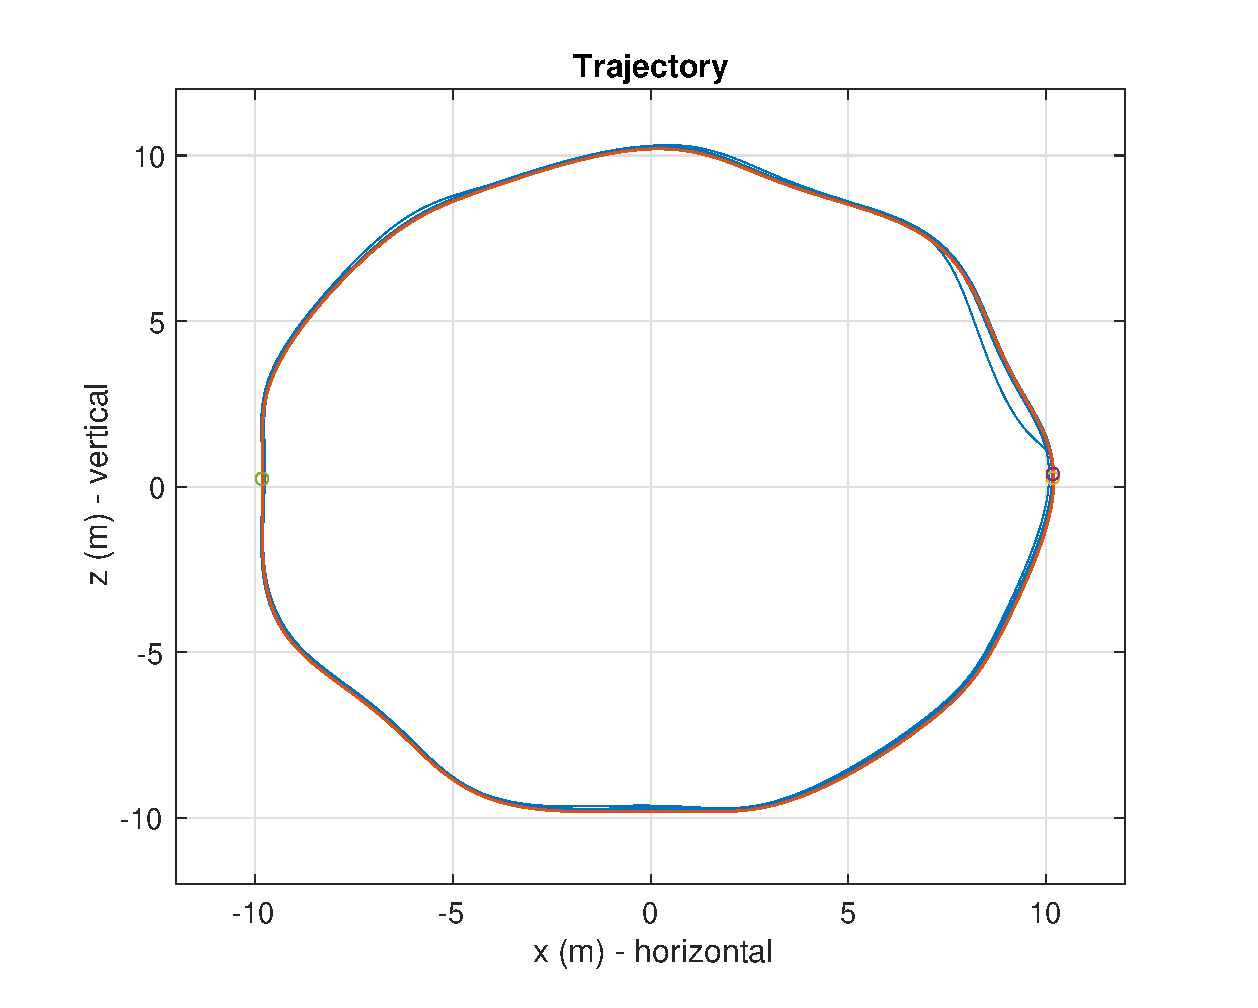
\includegraphics[width=\textwidth]{circle_full_controller_traj}
	\caption{Tandem-rotor vehicle trajectory - 15 ``laps'' with adaptation}
	\label{circle_traj_1}
\end{figure}	
\end{column}
\begin{column}{0.63\textwidth}
	\begin{figure}[h!]
	\centering
	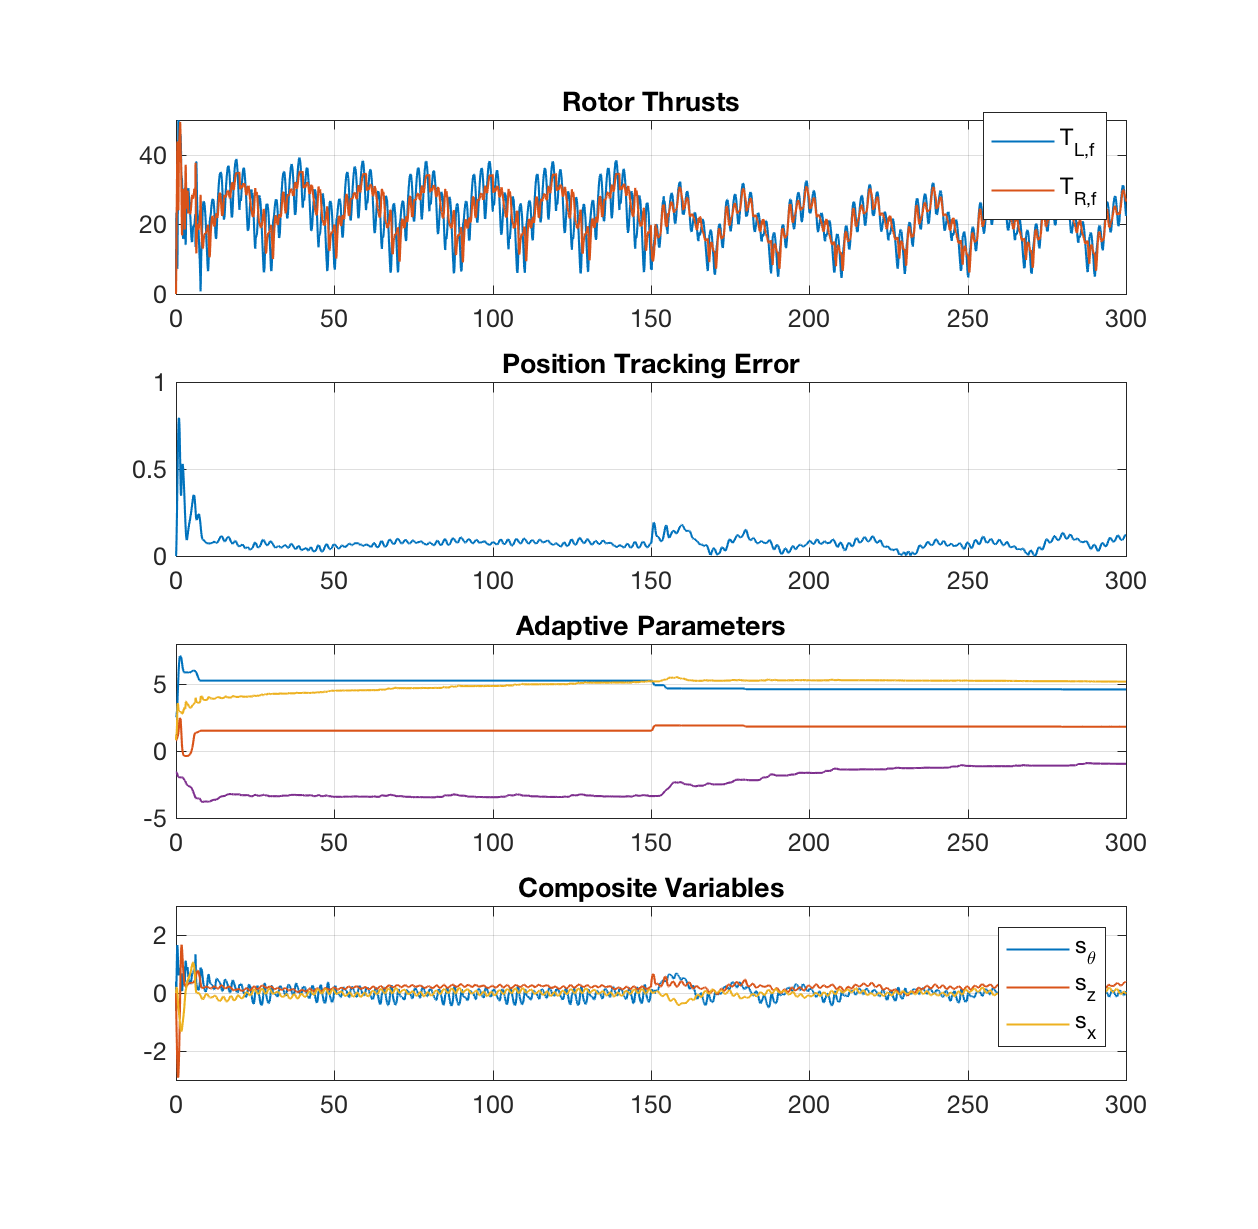
\includegraphics[width=\textwidth]{circle_full_controller} 
	\caption{Simulation results}
	\label{circle_data_1}
\end{figure}
\end{column}
\end{columns}
\normalsize
}


%--------------------------------------------------------------
\frame{\frametitle{Numerical Simulation}
%--------------------------------------------------------------
\footnotesize
\begin{columns}
\begin{column}{0.37\textwidth}
\begin{figure}[h!]
	\centering
	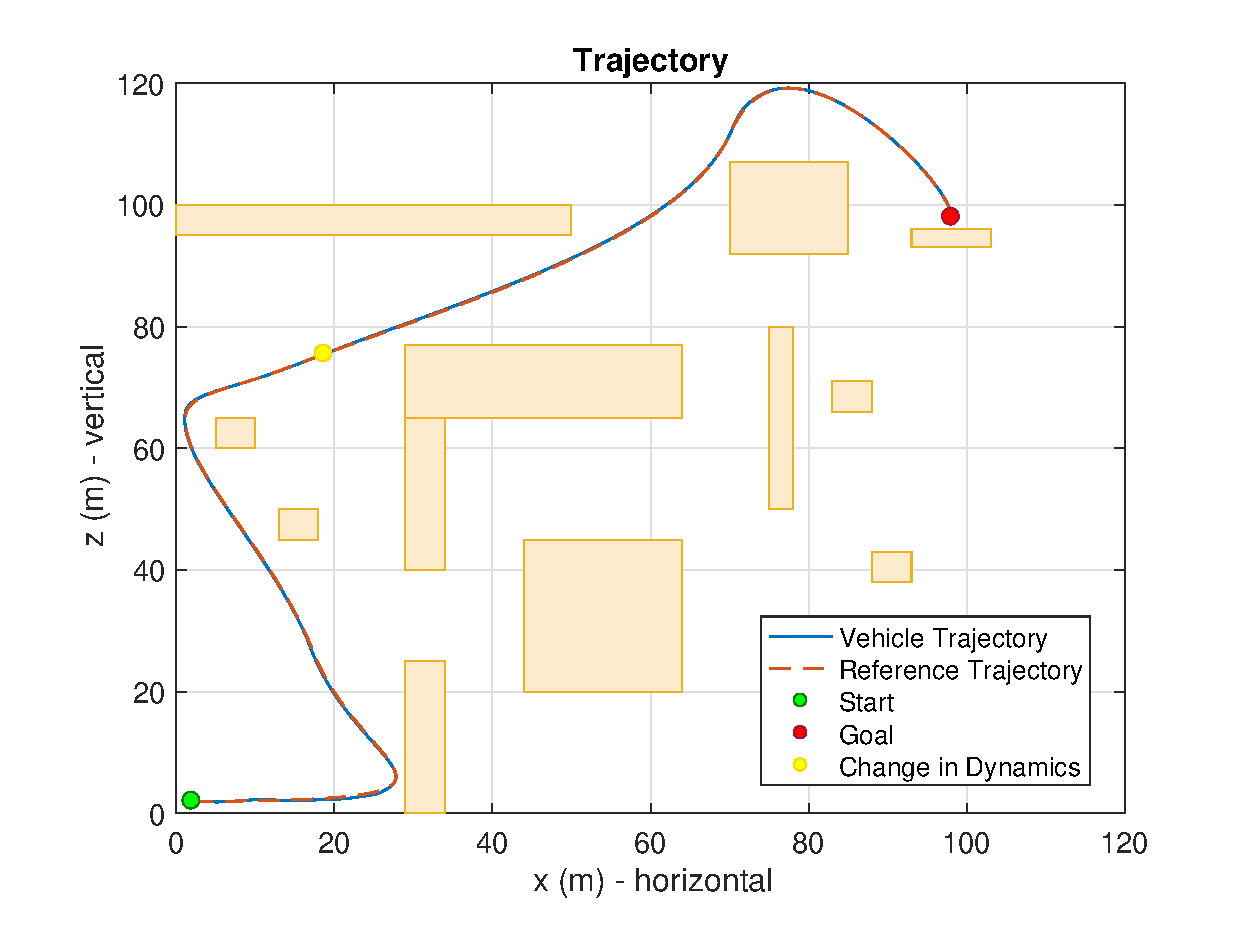
\includegraphics[width=\textwidth]{traj2}
	\caption{Tandem-rotor vehicle trajectory}
	\label{traj1}
\end{figure}	
\end{column}
\begin{column}{0.63\textwidth}
	\begin{figure}[h!]
	\centering
	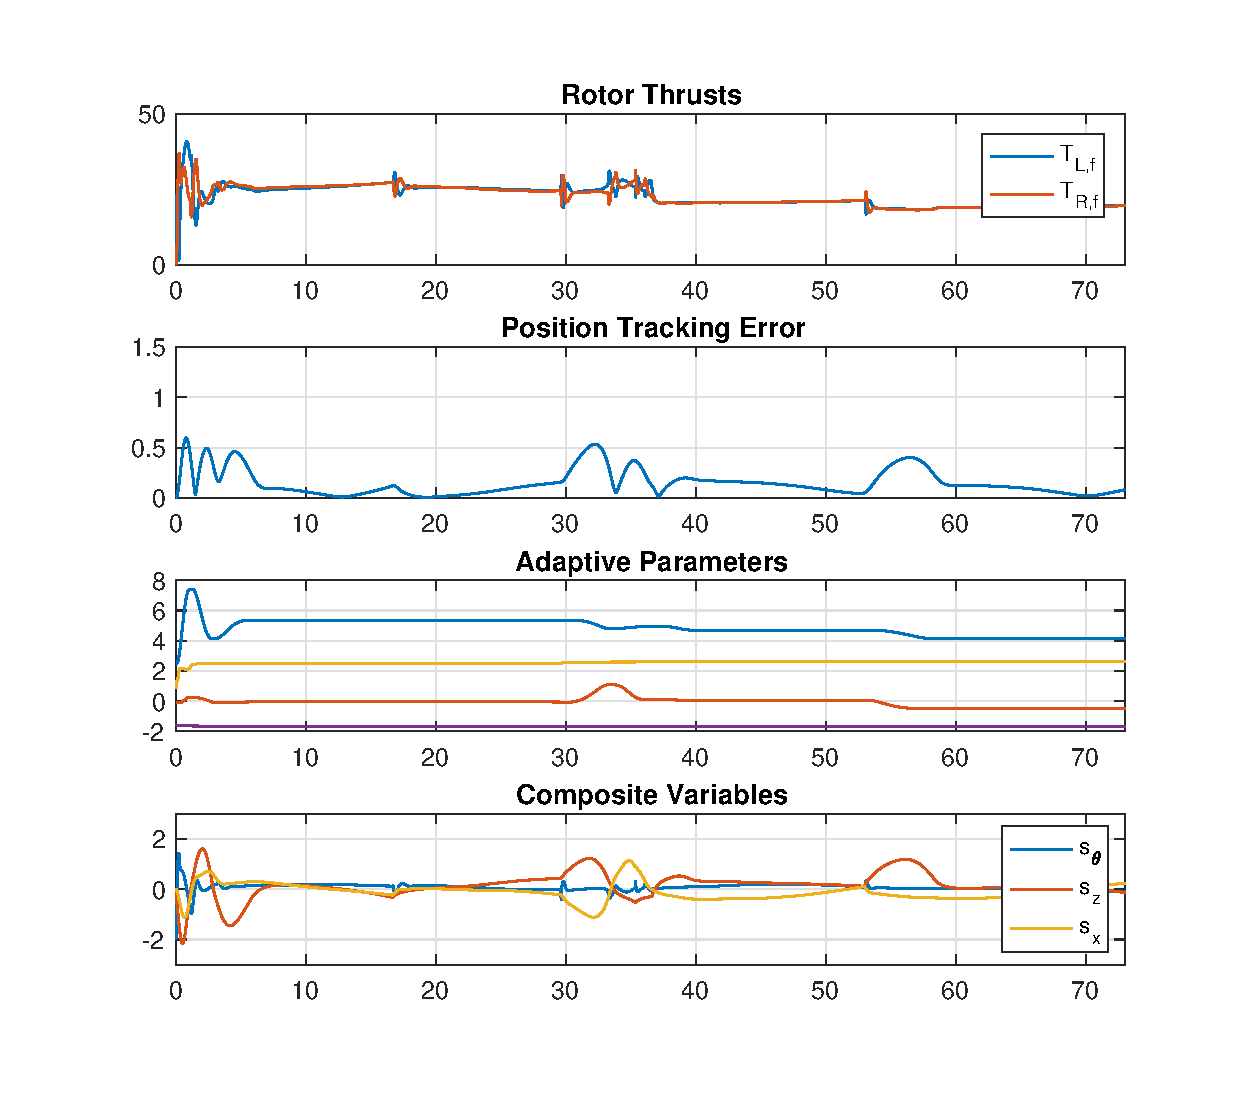
\includegraphics[width=\textwidth]{data3}
	\caption{Simulation results}
	\label{data1}
\end{figure}
\end{column}
\end{columns}
\normalsize
}

%--------------------------------------------------------------
\frame{\frametitle{Numerical Simulation - No Adaptation}
%--------------------------------------------------------------
\footnotesize
\begin{columns}
\begin{column}{0.37\textwidth}
\begin{figure}[h!]
	\centering
	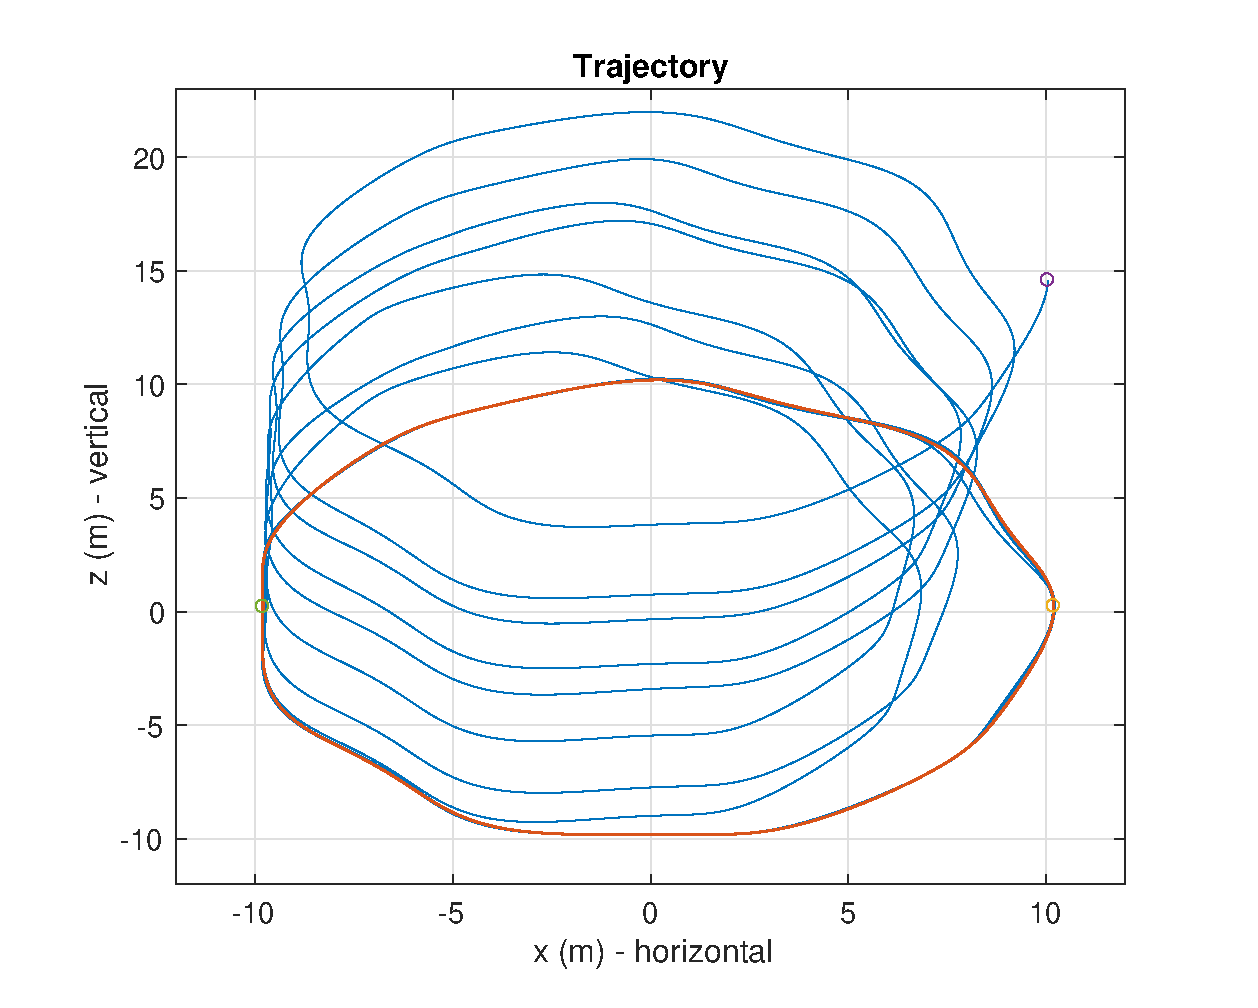
\includegraphics[width=\textwidth]{circle_noadap_traj}
	\caption{Tandem-rotor vehicle trajectory}
	\label{circle_traj_2}
\end{figure}	
\end{column}
\begin{column}{0.63\textwidth}
	\begin{figure}[h!]
	\centering
	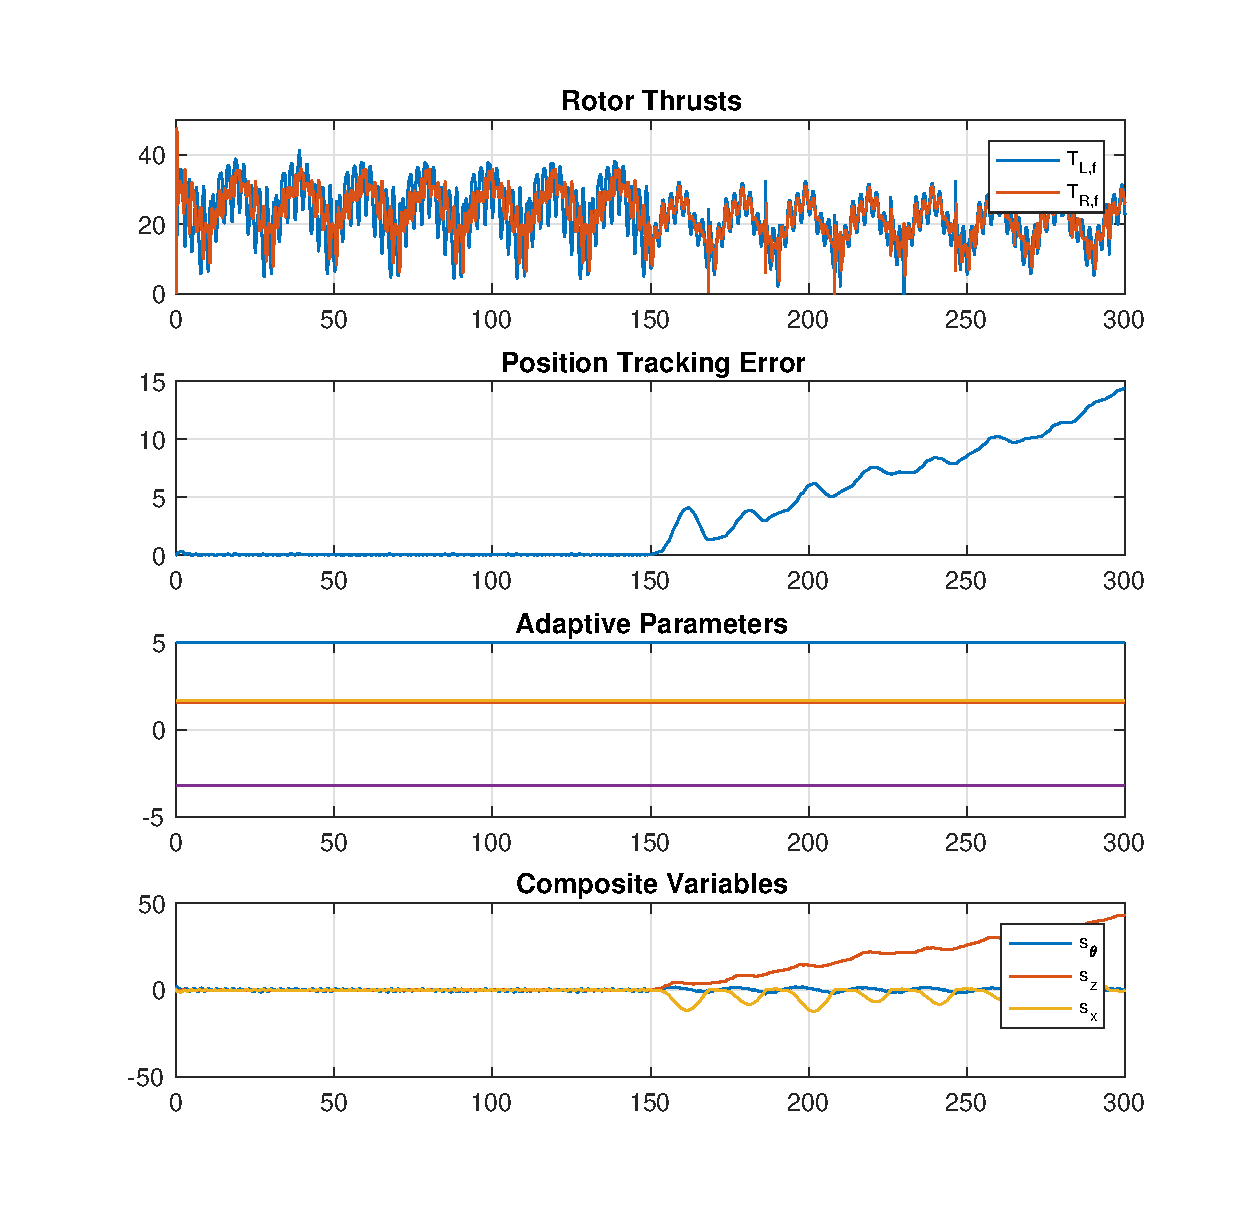
\includegraphics[width=\textwidth]{circle_noadap}
	\caption{Simulation results}
	\label{circle_data_2}
\end{figure}
\end{column}
\end{columns}
\normalsize
}

%--------------------------------------------------------------
\frame{\frametitle{Numerical Simulation - Linearized About Hover}
%--------------------------------------------------------------
\footnotesize
\begin{columns}
\begin{column}{0.37\textwidth}
\begin{figure}[h!]
	\centering
	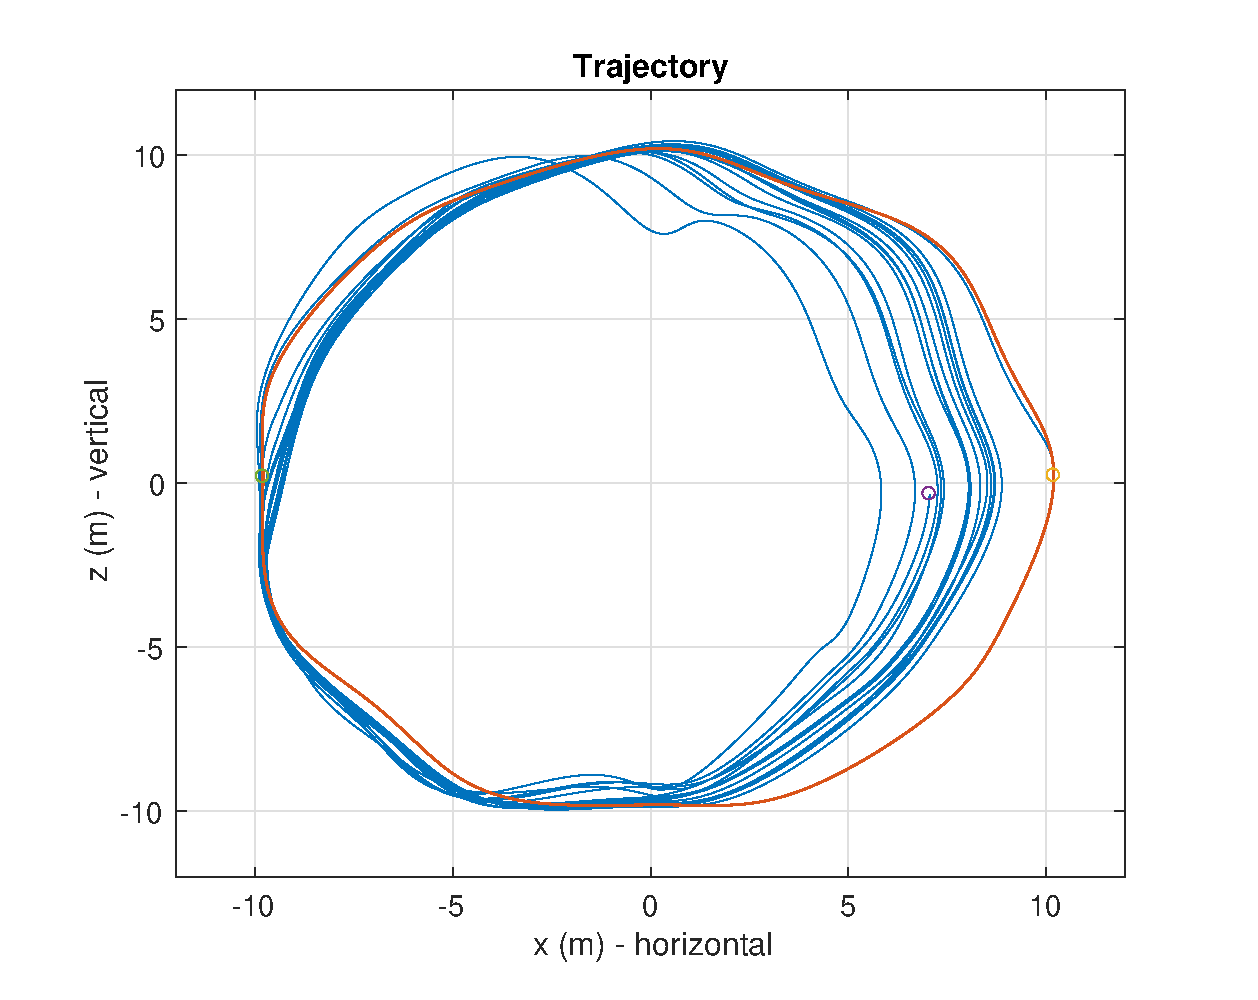
\includegraphics[width=\textwidth]{circle_linear_traj}
	\caption{Tandem-rotor vehicle trajectory}
	\label{circle_traj_3}
\end{figure}	
\end{column}
\begin{column}{0.63\textwidth}
	\begin{figure}[h!]
	\centering
	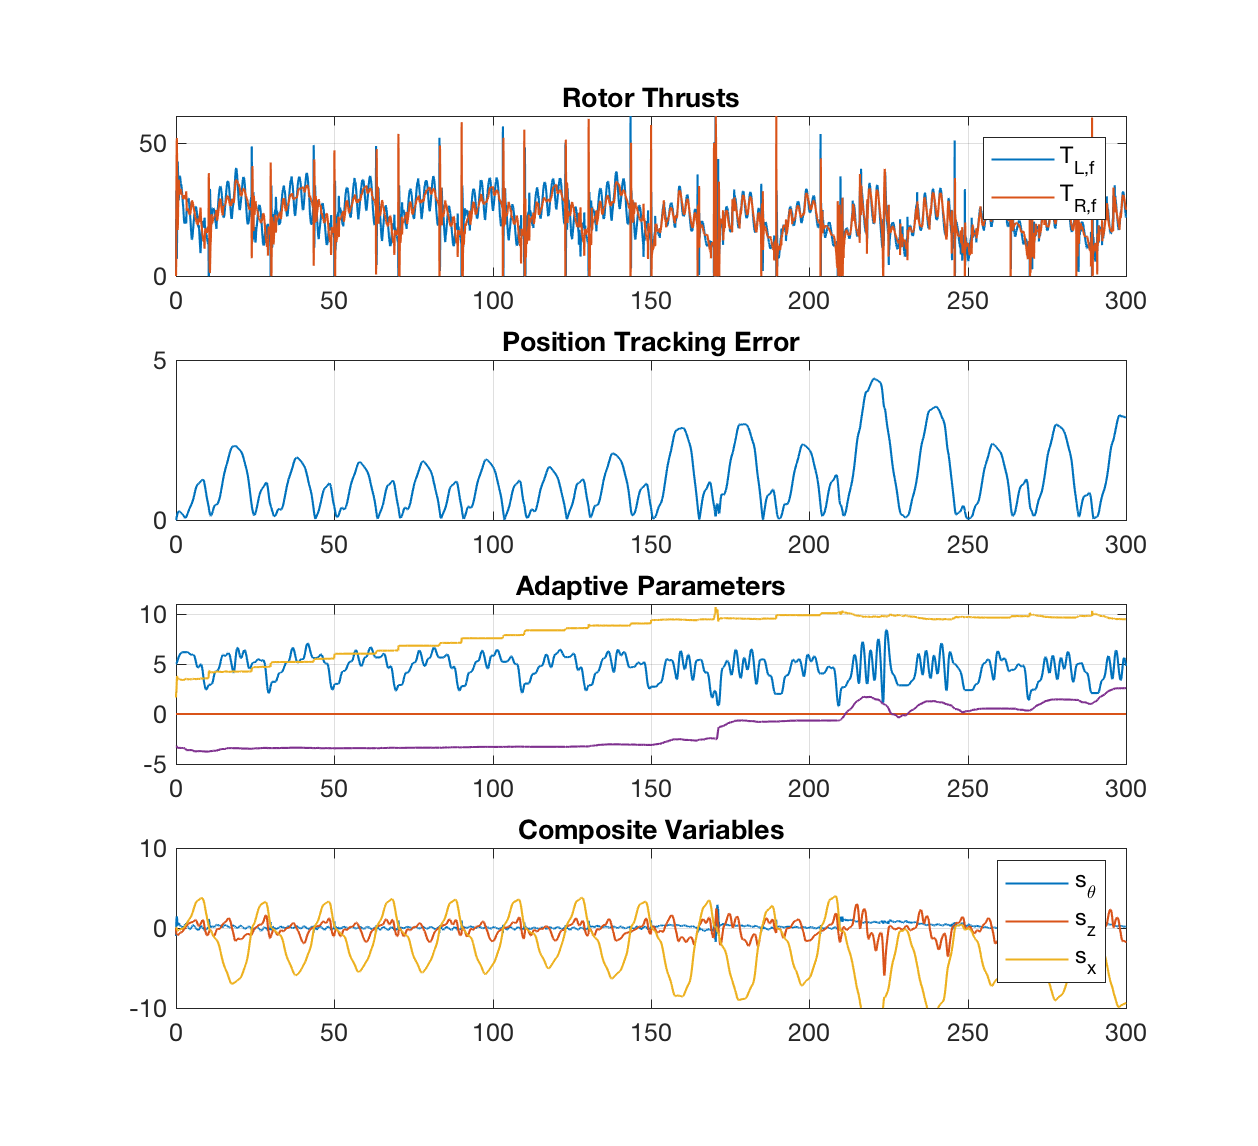
\includegraphics[width=\textwidth]{circle_linear}
	\caption{Simulation results}
	\label{circle_data_3}
\end{figure}
\end{column}
\end{columns}
\normalsize
}


%--------------------------------------------------------------
\frame{\frametitle{Summary}
%--------------------------------------------------------------
\footnotesize
\begin{columns}
\begin{column}{0.55\textwidth}
Conclusions:
\begin{itemize}
	\item Trajectory-tracking controller designed for planar quadrotor UAV with unknown parameters $m_p, \ell_p, \bar{c}_d, c_t$
	\item Ability to adapt online to changes in parameters demonstrated through simulations
	\item Adaptive controller shows robustness to unmodeled actuator dynamics and external disturbances
\end{itemize}
\end{column}
\begin{column}{0.45\textwidth}
Possible extensions:
\begin{itemize}
	\item Full dynamics of quadrotor UAV moving in 3D space
	\item Use vehicle parameters identified online to update kinodynamic motion plan
	\item Estimate slowly time-varying wind online
\end{itemize}
\end{column}
\end{columns}
\vspace{1.5cm}
\Large
\pause Thanks for listening! Questions?
\normalsize
}

%---------------------------------------------------------------------
\frame{\frametitle{References}
%----------------------------------------------------------------------
%\tiny
\nocite{slotine1991applied, karaman2010optimal, webb2013kinodynamic, allen2015toward, bouabdallah2007full}
%\bibliographystyle{ieeetr}
%\bibliography{feb1_bib}

%\bibliographystyle{authordate1}}
\printbibliography
}


%------------------%
\end{document}
%------------------%